\chapter{Part I(d) - ISA Arrays and Data Structures - W 2.2}
\section{Arrays}
\textit{In higher level languages, are written like follows :}
\begin{java}
short\[\] myData = \{10407, -16533, -22715, 29796, 18956, \dots\}:
\end{java}
\subsection{Different Ways to Store Arrays}
\begin{center}
    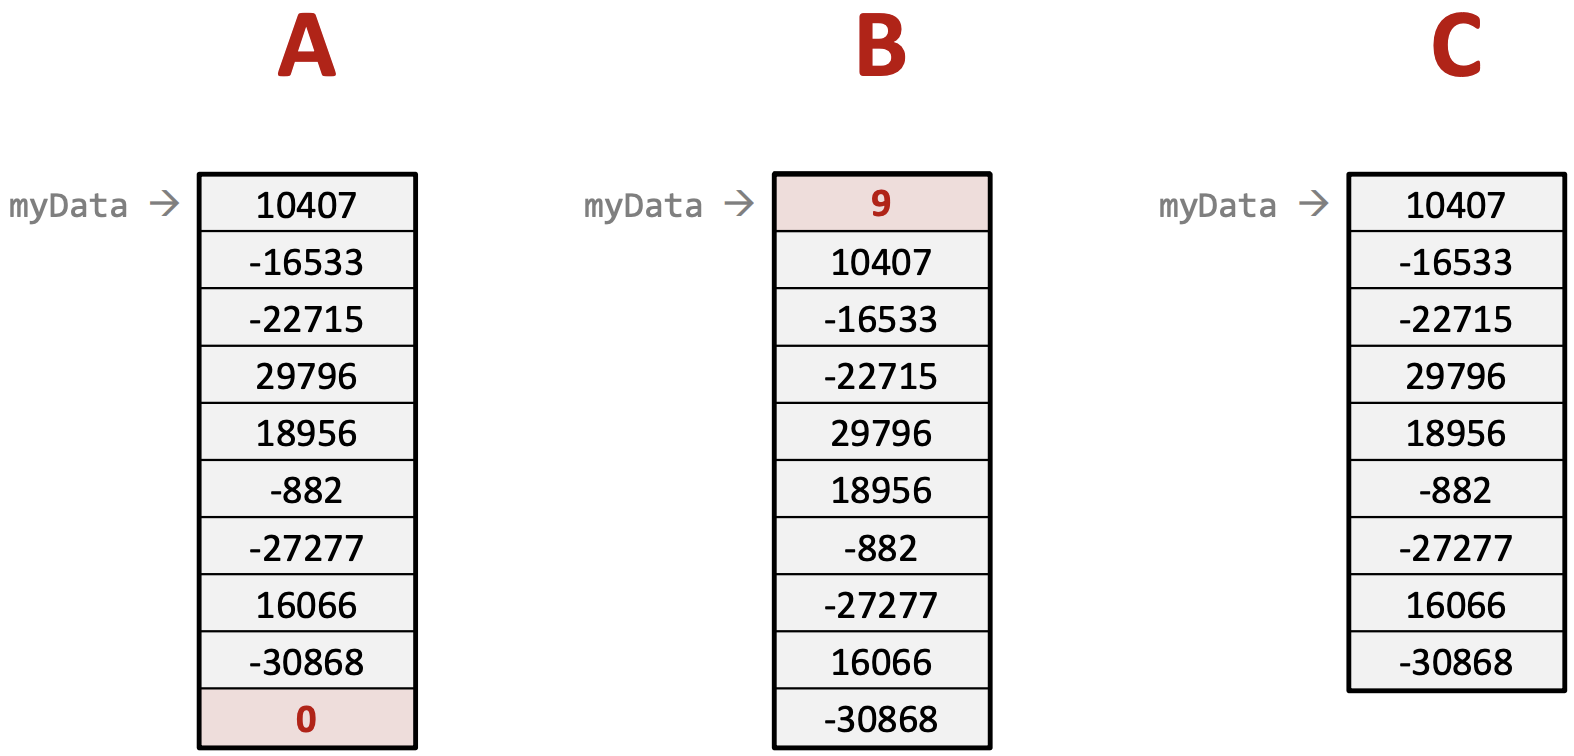
\includegraphics[width=0.45\textwidth]{chapters/chapter1d/images/arrays.png}
\end{center}
\begin{itemize}
\item \textbf{A: Storing Arrays with a Null Terminator}
\begin{itemize}
    \item[-] In this method, the array is stored with each element represented using 16-bit integers.
    \item[-] A null terminator (the value 0) is used at the end of the array to indicate its termination.
    \item[-] This method is common when the array size is unknown in advance, and the null terminator acts as a signal to stop reading the data.
\end{itemize}

\item \textbf{B: Storing Arrays with a Length Prefix}
\begin{itemize}
    \item[-] Here, the first element of the array contains the length of the array, stored as a 16-bit integer (in this case, the length is 9).
    \item[-] The rest of the array is stored in consecutive memory locations, similar to method A.
    \item[-] This method allows the array size to be known before reading all the data, making it more efficient for some use cases.
\end{itemize}

\item \textbf{C: Storing Arrays without a Terminator or Length Prefix}
\begin{itemize}
    \item[-] In this case, the array is stored without a length prefix or a null terminator.
    \item[-] The size of the array must be known externally, either through the code or an external mechanism.
    \item[-] This method is the most compact but requires prior knowledge of the array's size.
\end{itemize}
\end{itemize}

\subsection{Adding Positive Elements}
\textit{Here we'll write the same program for the different ways of storing arrays.} \\
\textit{The program will add all positive elements of an array of signed 16-bit integers. At call time, a0 points to the array, at return time, a0 contains the result.} \\

\textbf{A: Storing Arrays with a Null Terminator}\\
\begin{center}
    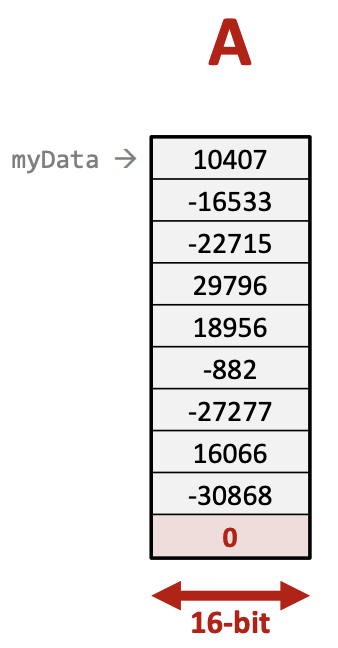
\includegraphics[width=0.14\textwidth]{chapters/chapter1d/images/A.png}
\end{center}

\begin{center}
\begin{assembly}
add_pos:li t0, 0         # Initialize t0 to 0
        lh t1, 0(a0)     # Load halfword from memory address a0 into t1
        beqz t1, end     # Branch to 'end' if t1 equals zero
        blez t1, donothing  # Branch to 'donothing' if t1 is less than or equal to zero
        add t0, t0, t1   # Add t1 to t0 (only if t1 is positive)
donothing:               # This block does nothing for negative or zero values
# You can put other operations here if needed
        j add_pos        # Jump back to the beginning of add_pos to check the next value
end:                     # Label 'end' for the program termination
\end{assembly}
\end{center}
\textbf{B: Storing Arrays with a Length Prefix} \\
\begin{center}
    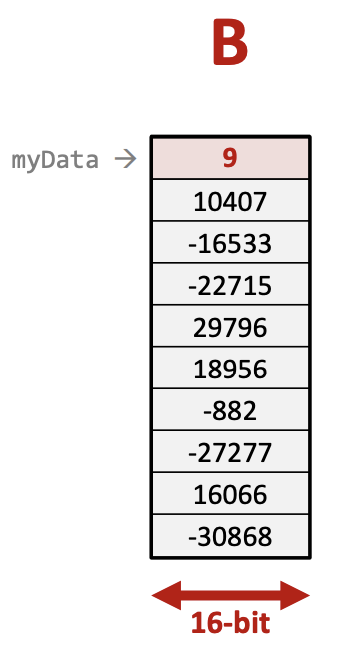
\includegraphics[width=0.14\textwidth]{chapters/chapter1d/images/B.png}
\end{center}

\begin{center}
\begin{assembly}
add_pos_b:  
    lh t2, 0(a0)        # Load the length of the array into t2
    addi a0, a0, 2      # Move to the first element of the array (skip the length prefix)
    li t0, 0            # Initialize t0 to 0 for storing the sum
loop_b:    
    beqz t2, end_b      # If the length (t2) is zero, branch to 'end_b'
    lh t1, 0(a0)        # Load the current array element into t1
    blez t1, skip_b     # If t1 is less than or equal to zero, skip the addition
    add t0, t0, t1      # Add t1 to t0 (only if t1 is positive)
skip_b:    
    addi a0, a0, 2      # Move to the next element in the array
    addi t2, t2, -1     # Decrease the length counter
    j loop_b            # Jump back to loop_b
end_b:                  # End label
\end{assembly}
\end{center}
\textbf{C: Storing Arrays without a Terminator or Length Prefix} \\
\begin{center}
    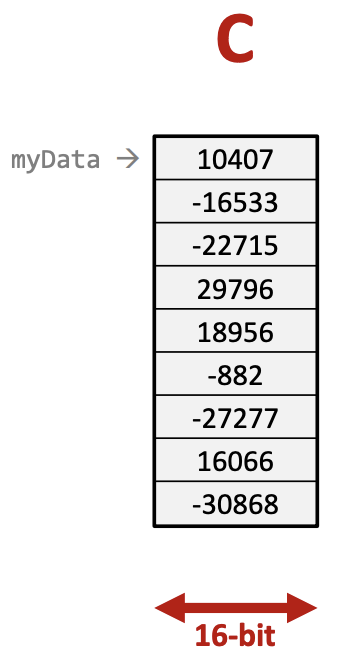
\includegraphics[width=0.14\textwidth]{chapters/chapter1d/images/C.png}
\end{center}

\begin{center}
\begin{assembly}
add_pos_c:  
    li t0, 0         # Initialize t0 to 0 for storing the sum
loop_c:     
    beqz t2, end_c   # If the array size (t2) is zero, branch to 'end_c'
    lh t1, 0(a0)     # Load the current array element into t1
    blez t1, skip_c  # If t1 is less than or equal to zero, skip the addition
    add t0, t0, t1   # Add t1 to t0 (only if t1 is positive)
skip_c:    
    addi a0, a0, 2   # Move to the next element in the array
    addi t2, t2, -1  # Decrease the array size counter
    j loop_c         # Jump back to loop_c
end_c:               # End label
\end{assembly}
\end{center}

\subsection{Pointer to Memory vs Index in Array}
\textit{Now we're wodnering which one of these two ways of accessing the array is better.} \\
\textbf{Obviously the less instructions the better (not always true actually but well),\\ Pointer to Memory.} \\
\begin{minipage}[htpb]{0.45\textwidth}
\begin{assembly}
add_positive:
    li t0, 0
    mv t1, a1
next_short:
    beq t1, zero, end
    lh t2, 0(a0)
    bltz t2, negative
    add t0, t0, t2
negative:
    addi a0, a0, 2
    addi t1, t1, -1
    j next_short
end:
    mv a0, t0
ret
\end{assembly}
\end{minipage}
\hfill
\vline
\hfill
\begin{minipage}[htp]{0.45\textwidth}
\begin{assembly}
add_positive:
    li t0, 0
    li t1, 0
next_index:
    bge t1, a1, end
    slli t2, t1, 1
    add t2, a0, t2
    lh t3, 0(t2)
    bltz t3, negative
    add t0, t0, t3
negative:
    addi t1, t1, 1
    j next_index
end:
    mv a0, t0
ret
\end{assembly}
\end{minipage}
\newpage
\subsubsection{In C}
\textit{Writing this in C for better understanding. Again, which one is better?} \\
\vspace*{5px}
\textbf{Obviously the less instructions the better (again not always true but ah), Index in array} \\
\begin{minipage}[htp]{0.45\textwidth}
\textbf{Pointer to memory} \\
\begin{cc}
short sum = 0;
short *ptr = myData;
short *end = myData + N;
while (ptr < end) {
    if (*ptr > 0) {
    sum += *ptr;
}
    ptr++;
}
\end{cc}
\end{minipage}
\hfill
\vline
\hfill
\begin{minipage}[htp]{0.45\textwidth}
\textbf{Index in array} \\
\begin{cc}
short sum = 0;
int i;
for (i = 0; i < N; i++) {
    if (myData[i] > 0) {
    sum += myData[i];
}
}
\end{cc}
\end{minipage}

\subsubsection{We need a good compiler}
\textit{Seeing this, the idea would be to have a sufficiently good \textbf{compiler} (check I.4.3.2 if needed) such that we write our C code in Index in array, and we get Pointer to memory code in assembly. Thus writing better code but also getting better performance.} \\
\textbf{Another type of collection we could've used to store the data is a \textit{Linked List}.} \\
\vspace*{5px}
\begin{minipage}[htp]{0.45\textwidth}   
    \textit{Linked lists are useful for efficiently inserting and deleting elements, especially in the middle of the list.} \\
    \vspace*{5px}
    \textit{Each 32-bit element in a linked list contains 16 bits for the value and 16 bits for the address of the next element, enabling efficient insertions but slower sequential access compared to arrays.}
\end{minipage}
\hfill
\vline
\hfill
\begin{minipage}[htp]{0.45\textwidth}
\begin{center}
    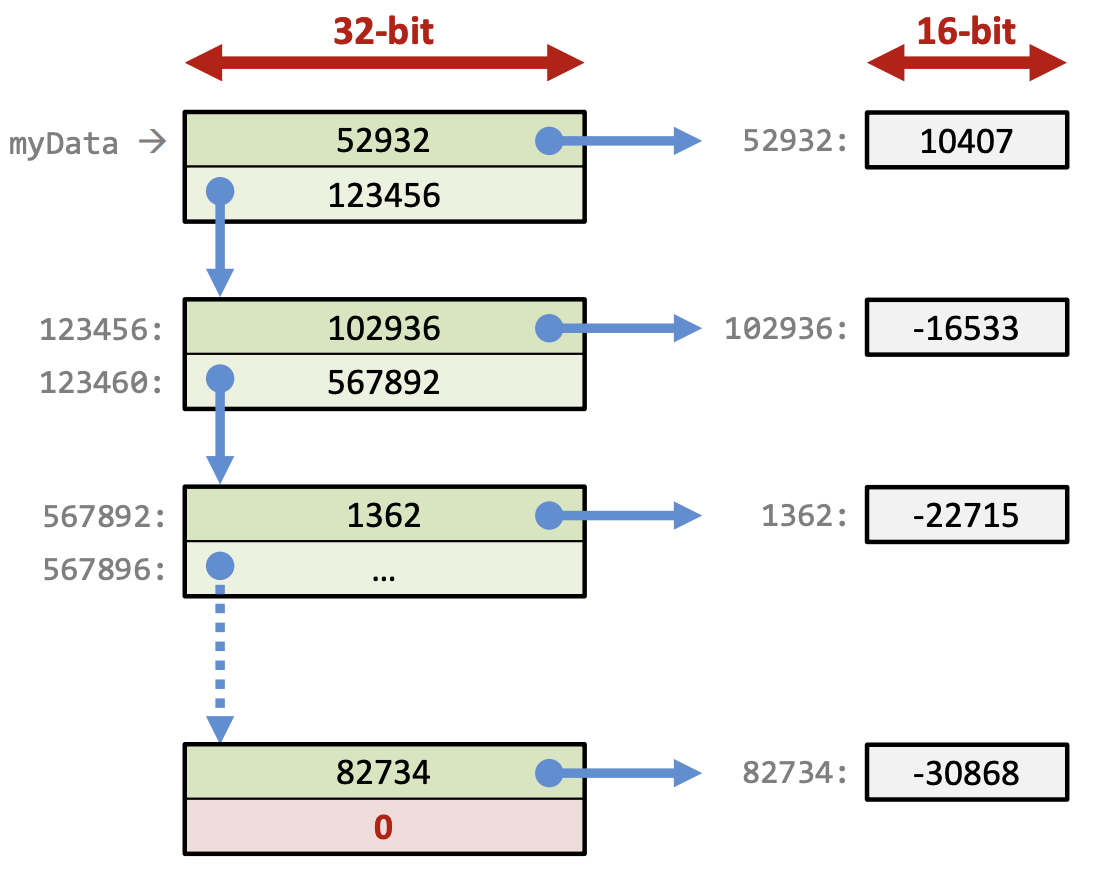
\includegraphics[width=0.95\textwidth]{chapters/chapter1d/images/linked_list.png}
\end{center}
\end{minipage}